\begin{figure*}[t]
    \centering
    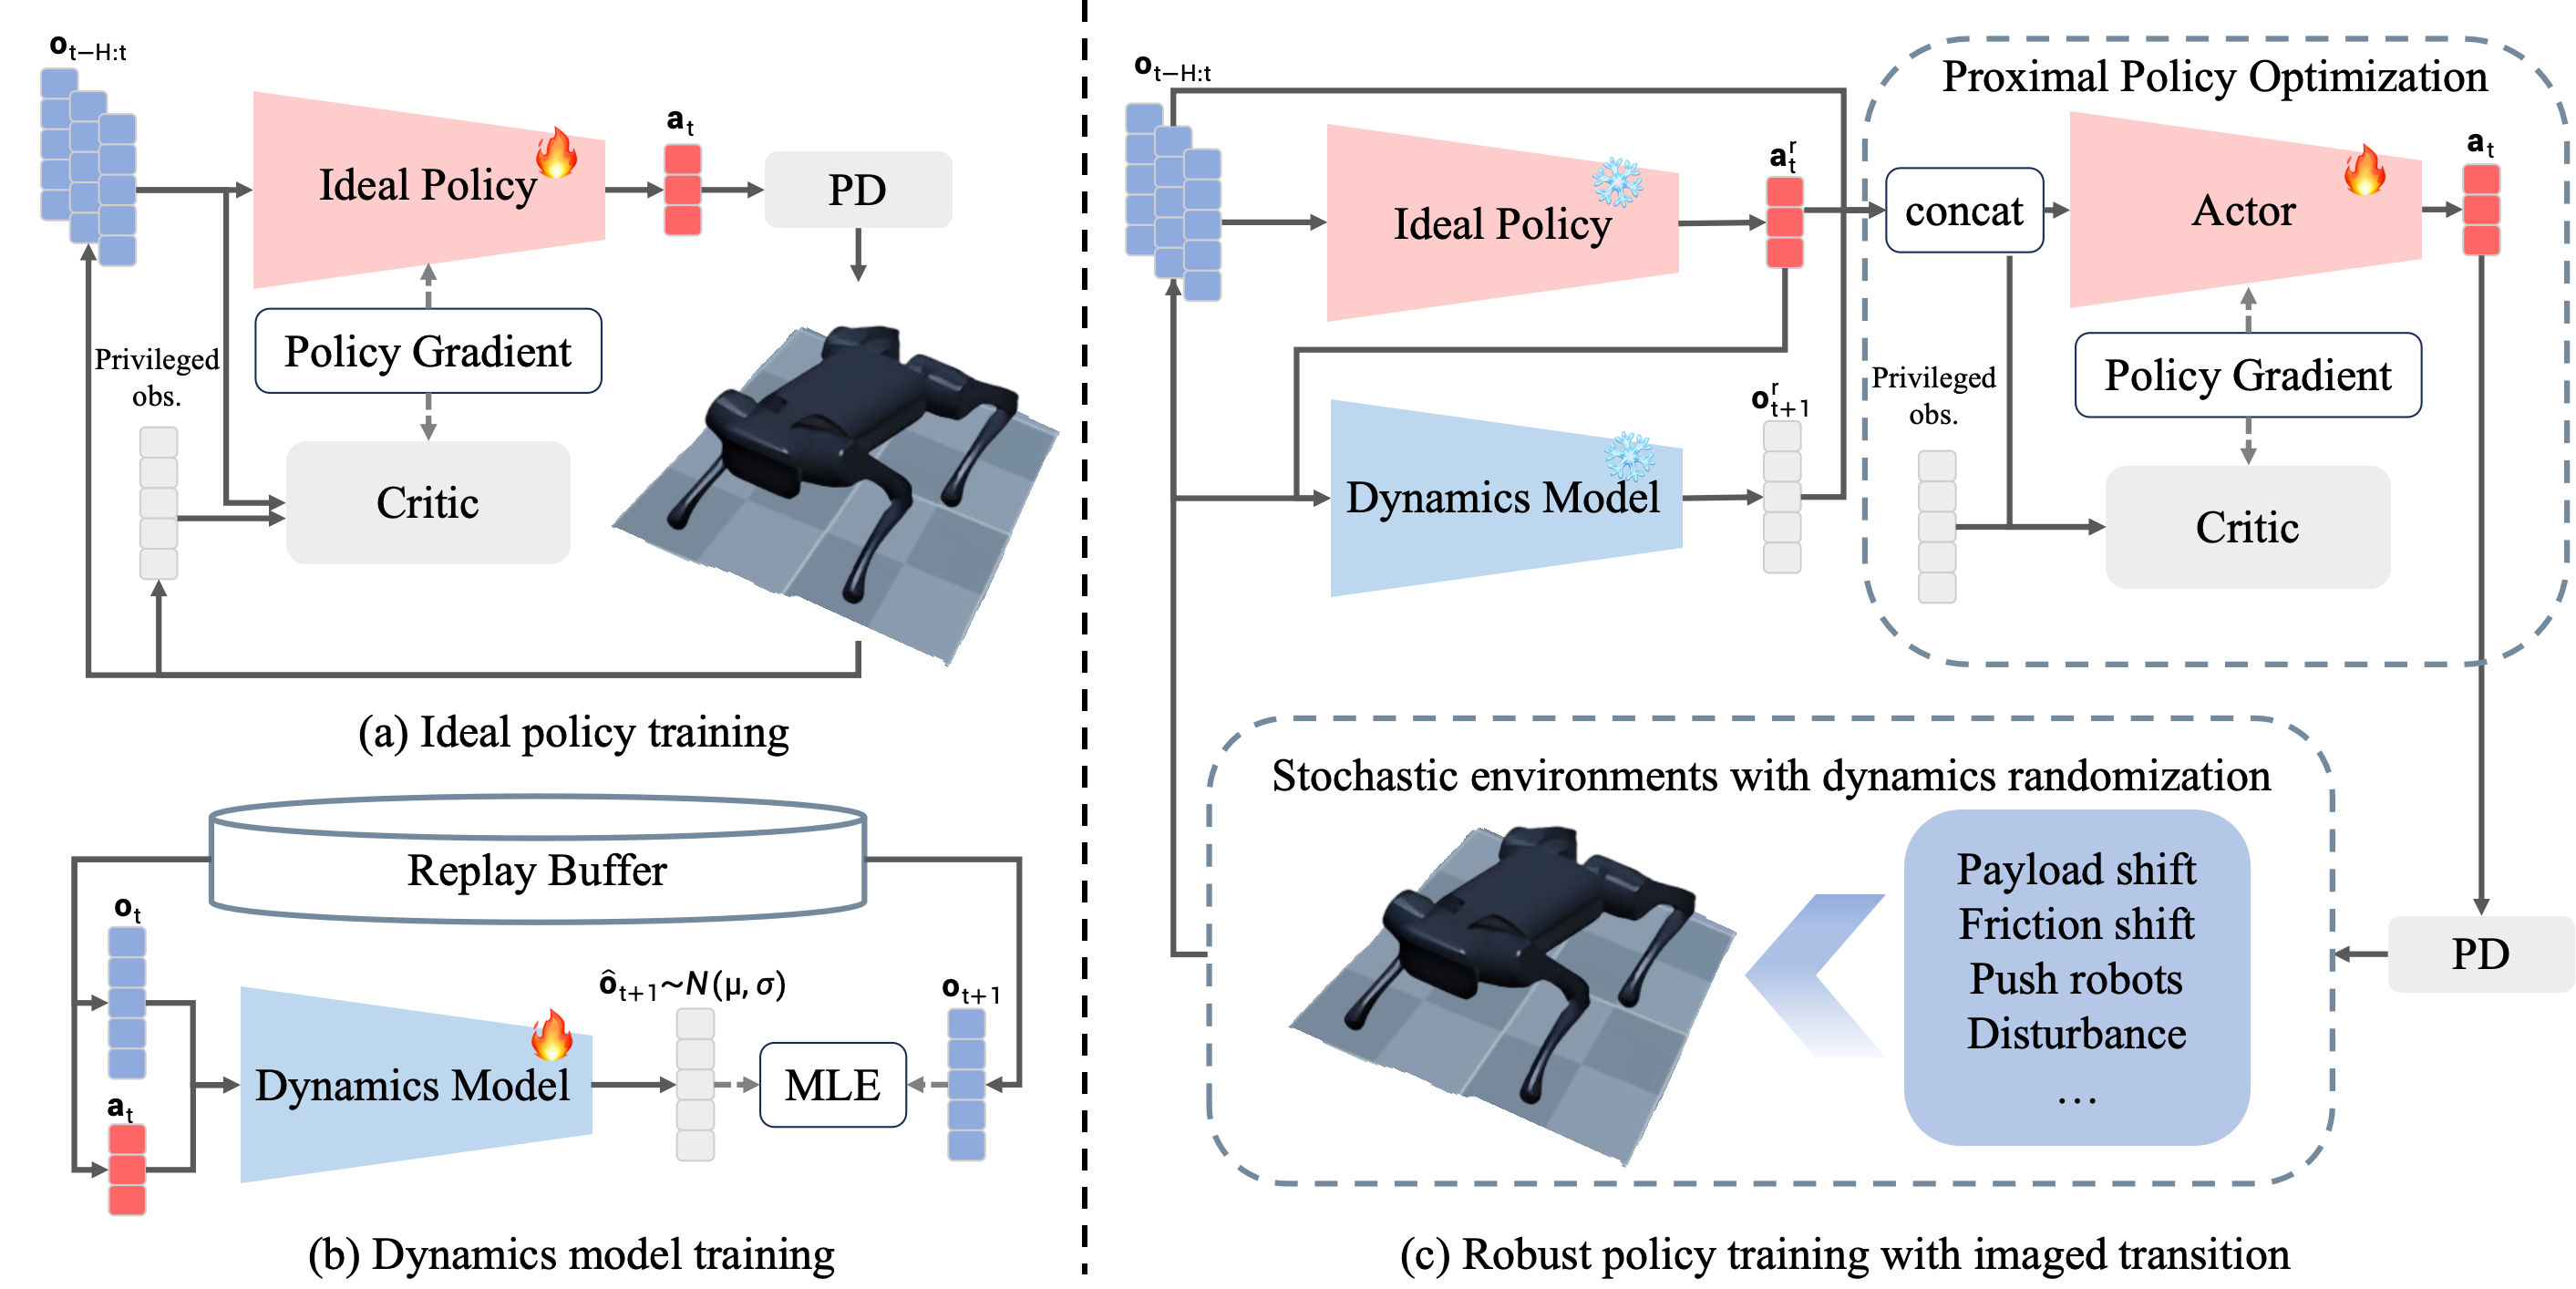
\includegraphics[width=1\linewidth]{fig/framework-min.png}
    \caption{\textbf{Framework Overview of LIT.} The left part is motion reference learning in fixed dynamics. The right part is policy learning with imagined transition. $\mathbf{a}^{r}_{t}$ and $\mathbf{o}^{r}_{t+1}$ mean reference action and imagined next observation respectively. $[\mathbf{o}_{t}, \mathbf{a}^{r}_{t}, \mathbf{o}^{r}_{t+1}]$ constitutes the imagined transition}
    \label{fig:framework}
\end{figure*}

\paragraph{POMDP} 
In this study, the environment is modeled as an infinite-horizon partially observable Markov decision process (POMDP), represented by the tuple \( \mathcal{M} = (\mathcal{S}, \mathcal{O}, \mathcal{A}, d_0, p, r, \gamma) \). The full state \( s \in \mathcal{S} \), partial observation \( o \in \mathcal{O} \), and action \( a \in \mathcal{A} \) are all continuous variables. The system begins with an initial state distribution, denoted by \( d_0(s_0) \), and evolves according to the state transition probability \( p(s_{t+1} | s_t, a_t) \). Each state transition yields a reward determined by the reward function \( r: \mathcal{S} \times \mathcal{A} \to \mathcal{R} \), while the discount factor is specified by \( \gamma \in [0, 1) \).
Additionally, we define a temporal observation at time \( t \) over the previous \( H \) time steps as \( \mathbf{o}_{t-H:t} = \left[ \mathbf{o}_t \quad \mathbf{o}_{t-1} \quad \cdots \quad \mathbf{o}_{t-H} \right]^T \). This representation captures the history of partial observations within the temporal window, which is crucial for decision-making in partially observable settings.

\paragraph{State Space}  
The policy network takes partial observations \(\mathbf{o}_{t}\) as input, which consist of the desired velocity, proprioceptive data from the joint encoders and IMU, as well as the previous action \(\mathbf{a}_{t-1}\). The IMU provides the base angular velocity \(\mathbf{\omega}_t\) and the gravity direction in the robot's frame of reference, denoted by \(\mathbf{g}_t\). The desired velocity, \(\mathbf{c}_t = [v_x^c, v_y^c, \omega_{\text{yaw}}^c]\), represents the linear velocities in the longitudinal and lateral directions, as well as the angular velocity around the yaw axis. The joint encoders supply the joint position \(\mathbf{\theta}_t\) and the joint velocity \(\dot{\mathbf{\theta}}_t\).
In the training phase, the critic network is granted access to privileged information, enabling it to provide more accurate state value estimations. The input to the critic network, \(\mathbf{o}_{t}^{c}\), includes three additional components compared to the actor network's input \(\mathbf{o}_{t}^{a}\): the current velocity \(\mathbf{v}_t\), the external force \(\mathbf{f}_t\), and the surrounding ground height \(\mathbf{h}_t\).

% \begin{equation}
%   \mathbf{o}_t=\begin{bmatrix}\boldsymbol{\omega}_t & \mathbf{g}_t & \mathbf{c}_t & \boldsymbol{\theta}_t & \boldsymbol{\dot{\theta}}_t & \mathbf{a}_{t-1} \end{bmatrix}^T,
%     \label{eq:actor_obs}
% \end{equation}
% \begin{equation}
%     \mathbf{o}_{t}^{c} = \begin{bmatrix}{\mathbf{o}_{t}, \mathbf{v}_{t}, \mathbf{f}_{t}, \mathbf{h}_{t}}\end{bmatrix}^T,
%     \label{eq:critic_obs}
% \end{equation}


\paragraph{Action Space}  
The movement of each actuator is modeled as the difference between the target joint position, denoted as \(\mathbf{\theta}_{\text{target}}\), and the nominal joint position, \(\mathbf{\theta}_0\). To mitigate the instability in the network's output, we introduce a scaling factor \(k \leq 1\) that is applied to the policy output \(\mathbf{a}_{t}\). Consequently, the final target joint positions are given by the equation:  
\(\mathbf{\theta}_{\text{target}} = \mathbf{\theta}_0 + k \mathbf{a}_{t}\).
The action space \(\mathcal{A}\) is defined by the number of actuators in the system. For instance, in the case of quadrupedal robots such as the Unitree A1, which is equipped with 12 actuators (3 on each leg), the dimension of the action space is 12.